\section{Response to Reviewer \#3}

Dear Reviewer 3,\\

Thank you very much for your thorough evaluation and valuable comments on our manuscript. We appreciate the reviewer's acknowledgement that the motivation is sound and the mathematical framework shows potential in enhancing LEO satellite communication reliability. Your detailed suggestions have been very helpful in improving the rigour and completeness of our work. We provide our detailed responses below.

\noindent\rule{17cm}{2.0pt}

%%%%%%%%%%%%%%%%%%%%%%%%%%%%%%%%%%%%%%%%%%%%%%%%%%%%%%%%%%%%%%%%%%%%%%
\subsection{Reviewer Comment-1}



\begin{mdframed}
\begin{quote}
The manuscript proposes a diversity-based OTFS system that integrates FEC with transmission diversity, supported by an ephemeris-driven framework for subchannel reliability prediction. In addition, it provides a rigorous finite-blocklength BLER analysis under various scenarios, including dominant-LOS, high-SNR, and Rayleigh fading conditions. While the motivation is sound and the mathematical framework shows potential in enhancing LEO satellite communication reliability, the overall contribution requires further clarification and improvement. Specific shortcomings regarding the system model assumptions, benchmarking, and presentation are summarized below.
1. In the manuscript, the reliability of each subchannel is inferred from outage probabilities derived based on large-scale fading, while the impact of small-scale fading appears to be marginalized. However, in satellite communication systems, multipath-induced frequency-selective fading and Doppler-induced fast time-varying fading can significantly affect the performance of FEC and diversity, especially in high-mobility scenarios. It is recommended that the authors explicitly incorporate the impact of small-scale fading into the reliability prediction analysis.


\end{quote}

\end{mdframed}


\subsection{Response}

We thank the reviewer for raising this point. Small-scale fading is incorporated into the proposed framework and analytically accounted for at every stage. In the channel model (Section~II-A), each tap gain includes a Rician small-scale component with $L_i$ multipath taps. In the BLER analysis (Section~III-A), Theorem~\ref{thm:fbl_bler} averages over the resulting fading distribution, and the closed-form approximation in Proposition~\ref{prop:bler_approx} expresses this average via the regularised incomplete gamma function, validated by simulation in Figs.~\ref{fig:prop1_validation} and~\ref{fig:prop2_diversity}. In the ephemeris predictor (Section~III-B), the predicted BLER evaluates this same expression at the predicted geometry, embedding the K-factor, diversity order $L_i$, and per-path NLOS power without requiring instantaneous CSI. Furthermore, a new SINR impairment model (Section~II-C) now accounts for fractional Doppler and imperfect channel estimation, validated in Fig.~\ref{fig:otfs_vs_ofdm}. A new footnote after Theorem~\ref{thm:fbl_bler} in Section~III-A also clarifies that the framework applies to any fading distribution, with the Rician-to-Nakagami-$m$ equivalence made explicit. We trace the role of small-scale fading through the paper's equations below.

\textbf{1) Channel model (Section~II-A).}
The channel model in~\eqref{eq:ntn_impulse_response} decomposes each tap gain into a large-scale and a small-scale Rician fading component:

\begin{quote}
``Each tap gain consists of a large-scale path-loss component and a small-scale Rician fading term, given by
$\alpha_{i,k\ell,p}(t) = \sqrt{G_{i,k\ell,\mathrm{LS}}(t) \cdot P_{i,k\ell,p}}\, g_{i,k\ell,p}(t),$
$\ldots$ The small-scale fading coefficient is modelled as''
\begin{equation*}
g_{i,k\ell,p}(t) = \sqrt{\frac{K_{i,k\ell}}{K_{i,k\ell}+1}}\,
e^{j2\pi f_{D,i,k\ell,p}t} + \sqrt{\frac{1}{K_{i,k\ell}+1}}\,
w_{i,k\ell,p}(t),
\end{equation*}
``where $K_{i,k\ell}$ denotes the Rician factor, $f_{D,i,k\ell,p}$
is the Doppler shift of tap $p$, and
$w_{i,k\ell,p}(t)\sim\mathcal{CN}(0,1)$ is the diffuse multipath
component.''
\end{quote}

The combined end-to-end SNR after MRC across the $L_i$ resolved access-link paths is given by~\eqref{eq:combined_snr_approx}:

\begin{quote}
\begin{equation*}
\gamma_i^{\mathrm{c}}(t) \approx \gamma_{i,\mathrm{SU}}^{\mathrm{MRC}}(t) = \bar{\gamma}_{i,\mathrm{SU}}(t) \sum_{p=0}^{L_i-1} P_{i,\mathrm{SU},p} \cdot |g_{i,\mathrm{SU},p}(t)|^2.
\end{equation*}
\end{quote}

\noindent where $|g_{i,SU,p}(t)|^2$ is the instantaneous small-scale fading power of the $p$th path. This SNR is a random variable whose distribution is governed by the small-scale fading statistics: the LOS component contributes the deterministic term $\gamma_{i,0}^{\mathrm{det}}$ from~\eqref{eq:los_deterministic}, while the $L_i - 1$ NLOS paths contribute the gamma-distributed random variable $\gamma_i^{\mathrm{NLOS}}$ from~\eqref{eq:nlos_aggregate}:

\begin{quote}
\begin{equation*}
\gamma_i^{\mathrm{c}}(t) = \gamma_{i,0}^{\mathrm{det}} + \gamma_i^{\mathrm{NLOS}}(t),
\end{equation*}
``$\ldots$ $\gamma_i^{\mathrm{NLOS}}$ follows a gamma distribution with shape parameter $L_i - 1$ and scale parameter $\hat{\gamma}_{i,\mathrm{NLOS}}$.''
\end{quote}

\textbf{2) Finite-blocklength BLER analysis (Section~III-A).}
The per-subchannel BLER in Theorem~\ref{thm:fbl_bler} averages over the small-scale fading distribution:

\begin{quote}
\begin{equation*}
\epsilon_i^{\mathrm{E2E}} = \mathbb{E}_{\gamma_i^{\mathrm{c}}}\left[Q\left(\frac{\sqrt{n_c}\left(C(\gamma_i^{\mathrm{c}}) - R_c\right) + \frac{\log_2 n_c}{2\sqrt{n_c}}}{\sqrt{V(\gamma_i^{\mathrm{c}})}}\right)\right],
\end{equation*}
``where the expectation is taken over the combined SNR $\gamma_i^{\mathrm{c}}$ with CDF given by~\eqref{eq:combined_cdf}.''
\end{quote}

The CDF in~\eqref{eq:combined_cdf} captures the small-scale fading distribution of the combined SNR:

\begin{quote}
\begin{equation*}
F_{\gamma_i^{\mathrm{c}}}(\gamma) = \Upsilon\left(L_i-1, \frac{\gamma - \gamma_{i,0}^{\mathrm{det}}}{\hat{\gamma}_{i,\mathrm{NLOS}}}\right), \quad \gamma \geq \gamma_{i,0}^{\mathrm{det}},
\end{equation*}
\end{quote}

\noindent Importantly, the BLER expression in Theorem~\ref{thm:fbl_bler} is general and applies to any fading distribution through the CDF of $\gamma_i^{\mathrm{c}}$. As noted in the footnote following Theorem~\ref{thm:fbl_bler}:

\begin{quote}
``{\color{blue}For Nakagami-$m$ fading, the CDF is the regularised lower incomplete gamma function $\Upsilon(m, \gamma/\bar{\gamma})$, and substituting this CDF into~\eqref{eq:bler_exact} recovers the Nakagami-$m$ FBL BLER directly. The Rician and Nakagami-$m$ distributions are related by $m = (K_{i,k\ell}+1)^2/(2K_{i,k\ell}+1)$; setting $K_{i,k\ell} = 0$ yields Rayleigh fading ($m = 1$), as shown in Corollary~\ref{cor:bler_rayleigh}.}''
\end{quote}

\noindent This demonstrates that the framework is not restricted to a single fading model; the same BLER expression accommodates Rician, Nakagami-$m$, and Rayleigh fading by substituting the appropriate CDF into~\eqref{eq:bler_exact}.

The closed-form BLER approximation in Proposition~\ref{prop:bler_approx} evaluates this expectation analytically:

\begin{quote}
\begin{equation*}
\epsilon_i^{\mathrm{E2E}} \approx F_{\gamma_i^{\mathrm{c}}}(\psi_i) = \Upsilon\left(L_i-1, \frac{\psi_i - \gamma_{i,0}^{\mathrm{det}}}{\hat{\gamma}_{i,\mathrm{NLOS}}}\right),
\end{equation*}
\end{quote}

This expression is a direct function of the small-scale fading parameters: the Rician K-factor (which determines the LOS/NLOS power split $P_{i,SU,0}$ and $P_{\mathrm{NLOS}}$), the number of resolvable multipath taps $L_i$ (which sets the shape parameter of the gamma distribution and thus the DD diversity order), and the per-path NLOS scale $\hat{\gamma}_{i,\mathrm{NLOS}}$. The simulation results in Fig.~\ref{fig:prop1_validation} and Fig.~\ref{fig:prop2_diversity} validate this analytical characterisation against simulation under both Rician and Rayleigh fading conditions:

\begin{center}
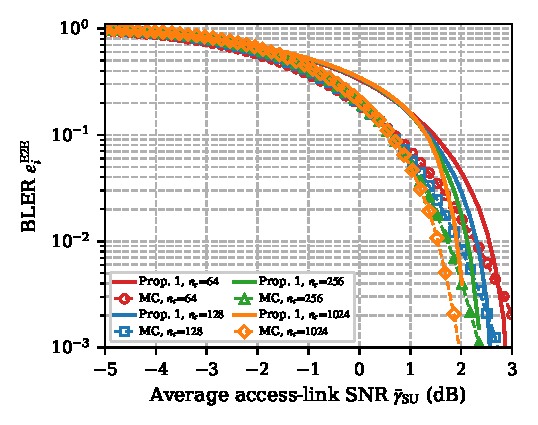
\includegraphics[width=0.7\columnwidth]{prop1_closedform_validation.eps}\\
{\small \textbf{Fig.~\ref{fig:prop1_validation}:} Subchannel BLER versus average access-link SNR for different blocklengths $n_c$ under dominant-LOS Rician fading: simulation and closed-form approximation in Proposition~\ref{prop:bler_approx}.}
\end{center}

\begin{center}
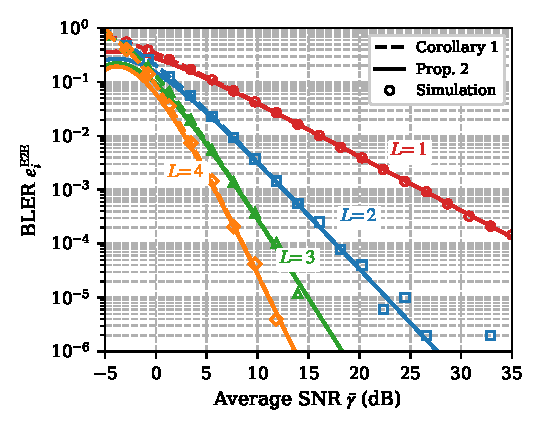
\includegraphics[width=0.7\columnwidth]{prop2_diversity_order.eps}\\
{\small \textbf{Fig.~\ref{fig:prop2_diversity}:} Subchannel BLER versus average access-link SNR for different DD diversity orders $L$ under Rayleigh fading: simulation, closed-form in Corollary~\ref{cor:bler_rayleigh}, and high-SNR asymptotic in Proposition~\ref{prop:bler_high_snr}.}
\end{center}

\textbf{3) Ephemeris-driven prediction (Section~III-B).}
The predicted BLER in~\eqref{eq:predicted_bler} uses the same closed-form expression from Proposition~\ref{prop:bler_approx}, evaluated at the predicted geometry:

\begin{quote}
\begin{equation*}
\tilde{\epsilon}_{i}^{\mathrm{E2E}}[k+\Delta] \approx \frac{1}{(L_i-1)!} \left(\frac{\psi_i - \tilde{\gamma}_{i,0}^{\mathrm{det}}[k+\Delta]}{\tilde{\hat{\gamma}}_{i,\mathrm{NLOS}}[k+\Delta]}\right)^{L_i-1} \times e^{-\frac{\psi_i - \tilde{\gamma}_{i,0}^{\mathrm{det}}[k+\Delta]}{\tilde{\hat{\gamma}}_{i,\mathrm{NLOS}}[k+\Delta]}}
\end{equation*}
\end{quote}

This predicted BLER is not based solely on large-scale fading. The parameters $L_i$, $\tilde{\gamma}_{i,0}^{\mathrm{det}}$, and $\tilde{\hat{\gamma}}_{i,\mathrm{NLOS}}$ embed the complete small-scale fading statistics: $L_i$ captures the multipath diversity order, the LOS/NLOS power split captures the Rician K-factor, and the regularised incomplete gamma function captures the probability that the instantaneous small-scale fading realisation causes the SNR to fall below the decoding threshold $\psi_i$. The predictor therefore accounts for the statistical impact of small-scale fading without requiring instantaneous CSI feedback, which is infeasible in mission-critical LEO NTN applications due to the long propagation delays.

\textbf{4) Impairment model for fractional Doppler and imperfect CSI (Section~II-C).}
In the revised manuscript, an explicit SINR model has been added for fractional Doppler (Doppler-induced fast time-varying fading) and imperfect channel estimation:

\begin{quote}
``{\color{blue}When the physical Doppler $\nu_p$ of the $p$th tap does not coincide
with a grid point, a fractional offset
$\alpha_p = \nu_p - \lfloor\nu_p\rceil$ introduces inter-Doppler
interference with variance
$\sigma_{\mathrm{frac}}^2 = (\pi\,\alpha_p)^2/(3\,N_{\mathrm{D}})$~\cite{Raviteja2018,Moose1994}.
Under imperfect channel estimation with per-element MSE
$\sigma_{\mathrm{CSI}}^2$, the effective post-equalisation SINR is}''
\begin{equation*}
\color{blue}
\gamma_i^{\mathrm{eff}} =
\frac{\gamma_i^{\mathrm{c}}}
{1 + \gamma_i^{\mathrm{c}}
\left(\sigma_{\mathrm{frac}}^2
+ \sigma_{\mathrm{CSI}}^2\right)}.
\end{equation*}
\end{quote}

Fig.~\ref{fig:otfs_vs_ofdm} validates this model, showing that both impaired OTFS curves exhibit a moderate BLER increase (approximately $1.5$--$2$ times) relative to the ideal integer-Doppler case, yet remain significantly below the OFDM curves at high normalised Doppler:

\begin{center}
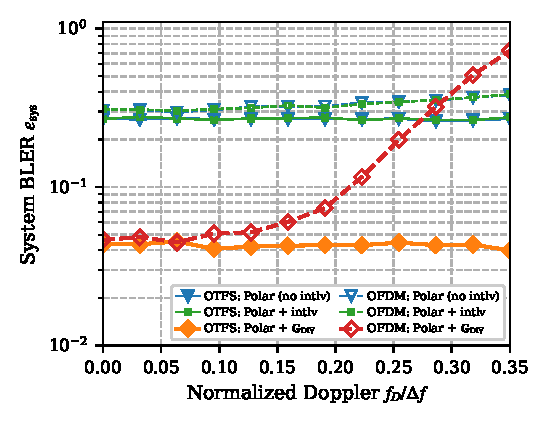
\includegraphics[width=0.7\columnwidth]{otfs_vs_ofdm.eps}\\
{\small \textbf{Fig.~\ref{fig:otfs_vs_ofdm}:} {\color{blue}BLER versus normalised Doppler $f_{D}/\Delta f$ for OTFS and OFDM at $P_{\mathrm{total}} = 20$~dBW, including fractional Doppler and imperfect channel estimation impairments.}}
\end{center}

In summary, the proposed framework incorporates small-scale fading at every stage: the channel model captures Rician multipath fading with $L_i$ resolvable taps (Eq.~\eqref{eq:ntn_impulse_response}--\eqref{eq:rician_fading}); the BLER analysis in Theorem~\ref{thm:fbl_bler} averages over the resulting fading distribution (Eq.~\eqref{eq:bler_exact}); the closed-form approximation in Proposition~\ref{prop:bler_approx} expresses this average analytically via the regularised incomplete gamma function (Eq.~\eqref{eq:bler_cdf_combined}), validated by simulation in Figs.~\ref{fig:prop1_validation} and~\ref{fig:prop2_diversity}; the ephemeris-driven predictor evaluates this same expression at the predicted geometry (Eq.~\eqref{eq:predicted_bler}); and the new SINR impairment model in~\eqref{eq:sinr_impairments} further accounts for frequency-selective and time-varying fading effects due to fractional Doppler and imperfect CSI (Fig.~\ref{fig:otfs_vs_ofdm}). The predictor uses statistical small-scale fading characterisation (K-factor, number of taps, per-tap power) rather than instantaneous CSI, since the latter is infeasible under the latency constraints of mission-critical LEO NTN applications.

We trust that this detailed tracing of small-scale fading through the analysis clarifies its role in the framework.


\subsection{Reviewer Comment-2}



\begin{mdframed}
\begin{quote}
The discussion of diversity techniques in the paper appears to be limited. The current work mainly compares the proposed scheme with conventional linear combining methods, such as SC and MRC. However, recent studies have explored more advanced diversity combining strategies, including robust combining, nonlinear combining, and AI-based approaches, which may offer improved performance under complex channel conditions. The authors should broaden the literature review and discussion on this aspect.

\end{quote}

\end{mdframed}


\subsection{Response}

We thank the reviewer for this suggestion. We agree that the literature review on diversity combining techniques should be broadened. In the revised manuscript, a new paragraph in the introduction discusses recent advanced receiver-side diversity strategies, including space-time block coded combining for multi-satellite systems~\cite{Singh2024}, model-driven deep learning detectors~\cite{He2020DL, Hu2023DL}, and adaptive deep learning-based receiver architectures~\cite{Doha2025}. The key distinction highlighted is architectural: these approaches all operate at the receiver side and combine copies of the same signal, whereas the proposed diversity transform operates at the transmitter side by algebraically mixing different coded content, providing a deterministic erasure recovery guarantee. In addition, MRC and SC baselines have been added to the latency figure (Fig.~\ref{fig:latency_comparison}) and rate-optimised MRC and SC to the throughput figure (Fig.~\ref{fig:throughput}), where the diversity transform surpasses MRC at $P_{\mathrm{total}} \approx 12$~dBW and achieves nearly twice the MRC throughput at 25~dBW. In the revised manuscript:

\begin{quote}
``$\ldots$ combining schemes such as SC and MRC effectively mitigate the probability of simultaneous deep fades, thereby enhancing link reliability~\cite{Cacuango2025}. {\color{blue}Beyond SC and MRC, recent studies have explored more advanced receiver-side diversity strategies, including space-time block coded combining for multi-satellite systems~\cite{Singh2024}, model-driven deep learning detectors that learn optimal signal combining from data~\cite{He2020DL, Hu2023DL}, and adaptive deep learning-based receiver architectures that learn to handle time-varying channel conditions without explicit mathematical models~\cite{Doha2025}. These techniques improve combining performance under complex channel conditions through learned or structured receiver processing. However, all of these approaches operate at the receiver side and combine multiple copies of the same transmitted signal. In contrast, the diversity transform proposed in this work operates at the transmitter side by algebraically mixing different coded content across subchannels prior to transmission, thereby providing a deterministic erasure recovery guarantee that receiver-side combiners alone cannot provide when an entire subchannel is erased.}''
\end{quote}

The updated throughput figure (Fig.~\ref{fig:throughput}) confirms these quantitative gains:

\begin{center}
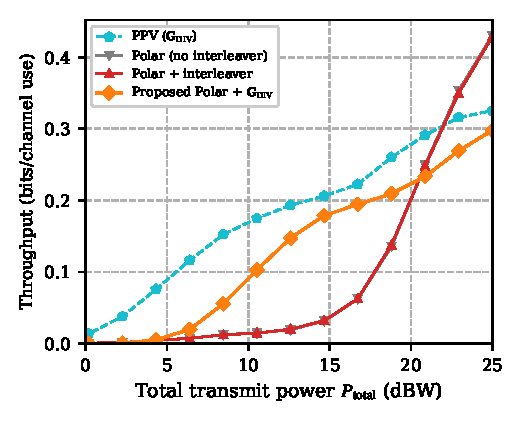
\includegraphics[width=0.7\columnwidth]{throughput_reliability.eps}\\
{\small \textbf{Fig.~\ref{fig:throughput}:} {\color{blue}Effective throughput versus total transmit power at $\epsilon = 40^{\circ}$ with $n_{\mathrm{s}} = 6$ subchannels. The diversity transform operates at effective rate $R_c \cdot \varrho/n_{\mathrm{out}} \approx 0.33$; per-subchannel baselines at $R_c = 0.5$. MRC and SC are rate-optimised at each power level.}}
\end{center}

We hope that the broadened literature review addresses this suggestion.


\subsection{Reviewer Comment-3}



\begin{mdframed}
\begin{quote}
The manuscript implies that the diversity transform matrix $G_{\mathrm{DIV}}$ is constructed based on time-varying outage patterns predicted by ephemerides. However, it does not clearly specify how $G_{\mathrm{DIV}}$ is updated dynamically at the physical layer. Furthermore, due to the different propagation distances between multiple satellites and the gateway, timing advance (TA) should be critically considered in the construction of the $G_{\mathrm{DIV}}$ matrix to ensure block-level synchronization among satellites.

\end{quote}

\end{mdframed}


\subsection{Response}

We thank the reviewer for this comment. The revised manuscript clarifies both points in Section~IV-F. First, the diversity transform matrix $G_{\mathrm{DIV}}$ is not recomputed dynamically: it is constructed once offline, and all $\binom{n_{\mathrm{s}}}{k_{\mathrm{c}}}$ recovery matrices are precomputed and stored in a lookup table; the only per-frame update is a table index selection based on the predicted outage set. Second, block-level synchronisation is ensured through per-subchannel timing advance at the gateway using ephemeris-derived slant ranges, following the standard 3GPP NTN procedure, so that all OTFS frames arrive block-aligned at the UE independently of the diversity transform construction. In the revised manuscript:

\textbf{1) Dynamic update of $G_{\mathrm{DIV}}$.}
The matrix $G_{\mathrm{DIV}}$ is not recomputed dynamically. It is constructed once offline from the RS--Vandermonde construction in Algorithm~\ref{alg:div_transform_construction}, and all $\binom{n_{\mathrm{s}}}{k_{\mathrm{c}}}$ recovery matrices are precomputed and stored in a lookup table. In Section~IV-F:

\begin{quote}
``{\color{blue}Since the MDS code parameters $(k_{\mathrm{c}}, n_{\mathrm{s}}, m)$
are fixed for a given system configuration, the matrix
$G_{\mathrm{DIV}}$ itself remains static across frames.
At each frame, the ephemeris-driven predictor in
Section~\ref{sec:ephemeris_prediction} computes per-subchannel
BLER estimates $\tilde{\epsilon}_{i}^{\mathrm{E2E}}$ and
identifies which subchannels exceed the erasure threshold
$\epsilon_{\mathrm{th}}$, producing the predicted outage set
$S_{\mathrm{out}}$ in~\eqref{eq:outage_set}. The receiver then
selects the corresponding precomputed recovery matrix from the
lookup table indexed by $S_{\mathrm{out}}$. Thus, the only
per-frame update is a table index selection, not a matrix
recomputation.}''
\end{quote}

\textbf{2) Timing advance and block-level synchronisation.}
The diversity transform operates on the algebraic data plane at the gateway, before transmission. The differential propagation delays between satellites are handled separately at the physical layer. In Section~IV-F:

\begin{quote}
``{\color{blue}Regarding block-level synchronisation across subchannels, the
diversity transform operates on the algebraic data plane at the
gateway, mapping encoded subwords to transform outputs before
transmission. The differential propagation delays between the
gateway and each satellite are deterministic functions of the
ephemeris-derived slant ranges in~\eqref{eq:slant_range} and are
pre-compensated at the gateway through per-subchannel timing
advance, following the standard 3GPP NTN timing advance
procedure~\cite{3GPP38821}. Consequently, the OTFS frames
arriving at the UE from different satellites are block-aligned,
and the diversity transform construction is independent of the
physical-layer timing.}''
\end{quote}

In summary, $G_{\mathrm{DIV}}$ is static and precomputed offline; only the active erasure pattern index changes per frame. Block-level synchronisation is ensured by per-subchannel timing advance at the gateway using ephemeris-derived slant ranges, following the 3GPP NTN procedure, and is decoupled from the diversity transform construction.

We trust that these clarifications resolve the concerns about dynamic update and timing.


\subsection{Reviewer Comment-4}



\begin{mdframed}
\begin{quote}
In the numerical results, the paper only considers polar codes for performance evaluation, without comparing against other widely adopted FEC schemes in satellite communication(e.g., LDPC or Turbo codes). Moreover, the performance under different code rates is not sufficiently explored. Since the effectiveness of the proposed joint framework may highly depend on the specific coding scheme and rate, the lack of such comparisons makes it difficult to assess the generality of the conclusions.
\end{quote}

\end{mdframed}


\subsection{Response}

We thank the reviewer for this important suggestion. In the revised manuscript, a new FEC comparison figure (Fig.~\ref{fig:fec_comparison}) has been added to Section~V that evaluates the proposed diversity transform with both polar codes (SCL decoding, list size~32) and LDPC codes (BP decoding, 50 iterations) at three code rates $R_c \approx 1/4$, $1/2$, and $3/4$. At each code rate, the polar and LDPC curves are nearly indistinguishable (residual gap below 0.2~dB), confirming that the system BLER is dominated by the MDS erasure recovery mechanism rather than by the specific FEC decoder. Per-subchannel no-diversity baselines at matching rates are included for reference. In the revised manuscript:

\begin{quote}
``{\color{blue}Fig.~\ref{fig:fec_comparison} demonstrates the FEC-agnostic operation of the proposed diversity transform by comparing polar codes (SCL decoding, list size~$32$) and LDPC codes (BP decoding, $50$ iterations) at three code rates $R_c \approx 1/4$, $1/2$, and $3/4$. All codes are combined with the diversity transform $\mathbf{G}_{\mathrm{DIV}}$ and evaluated under identical channel conditions. At each code rate, the polar and LDPC curves are nearly indistinguishable, with the residual gap remaining below $0.2$~dB across the entire power range. This confirms that the system BLER is dominated by the diversity transform's erasure recovery mechanism rather than by the specific FEC decoder, confirming FEC-agnostic operation. The diversity gain is largest at higher code rates: at $R_c = 3/4$, the no-diversity baseline remains above $0.25$ even at $P_{\mathrm{total}} = 23$~dBW, whereas the diversity-transform-equipped schemes reach $0.03$, because the weaker FEC protection makes the system more reliant on the erasure recovery provided by $\mathbf{G}_{\mathrm{DIV}}$. At $R_c = 1/4$, the stronger FEC narrows the gap, but the diversity transform still provides a consistent advantage across all power levels.}''
\end{quote}

\begin{center}
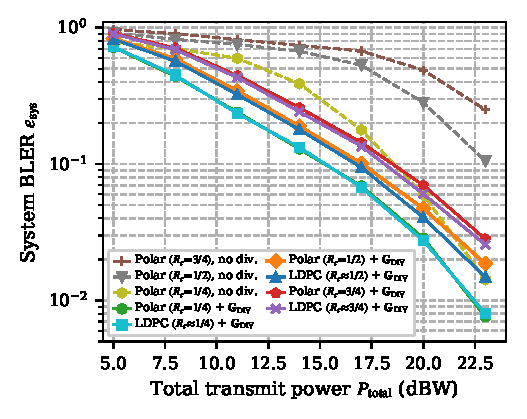
\includegraphics[width=0.7\columnwidth]{fec_comparison.eps}\\
{\small \textbf{Fig.~\ref{fig:fec_comparison}:} {\color{blue}System BLER versus total transmit power for polar and LDPC codes with the proposed diversity transform. No-diversity baselines shown for reference.}}
\end{center}

The summary paragraph in Section~V has also been updated to reflect these findings:

\begin{quote}
``$\ldots$ The combination of OTFS and the diversity transform maintains stable performance under high Doppler shifts where OFDM degrades significantly (Fig.~\ref{fig:otfs_vs_ofdm}). {\color{blue}The FEC comparison in Fig.~\ref{fig:fec_comparison} confirms that the diversity transform operates independently of the underlying FEC scheme: polar and LDPC codes achieve nearly identical BLER at all code rates when combined with $\mathbf{G}_{\mathrm{DIV}}$, indicating that the system performance is governed by the erasure recovery capability rather than the specific decoder.} Finally, single-shot decoding eliminates $\ldots$''
\end{quote}

Furthermore, the conclusion (Section~VI) now explicitly states the FEC-agnostic property:

\begin{quote}
``{\color{blue}The diversity transform also outperforms MRC, SC, and HARQ-CC across latency and throughput metrics, overcoming the fundamental spectral efficiency ceiling of repetition-based combining. The modular architecture is FEC-agnostic, enabling composition with any coding scheme without cross-layer redesign.}''
\end{quote}

The near-identical performance of polar and LDPC codes across three code rates validates the generality of the proposed framework: the diversity transform provides a deterministic erasure recovery layer that is independent of the underlying FEC scheme, consistent with the architectural decoupling established in Theorem~\ref{thm:block_mds}.

We trust that the new FEC comparison demonstrates the generality of the proposed framework.


\subsection{Reviewer Comment-5}



\begin{mdframed}
\begin{quote}
Although extensive simulations are presented, there appears to be a lack of comparison with existing integrated schemes. The authors are requested to benchmark their proposed architecture against recent relevant studies, rather than solely comparing it with isolated baseline components.

\end{quote}

\end{mdframed}


\subsection{Response}

We thank the reviewer for this comment. We agree that the manuscript should benchmark against integrated system-level schemes. In the revised manuscript, three categories of baselines have been added: (i) MRC and SC have been included in both the throughput (Fig.~\ref{fig:throughput}) and latency (Fig.~\ref{fig:latency_comparison}) comparisons, with MRC/SC rate-optimised to give their most favourable evaluation; (ii) a new FEC comparison (Fig.~\ref{fig:fec_comparison}) demonstrates that the architecture operates identically with polar and LDPC codes at all code rates; and (iii) the conclusion and summary paragraph have been updated to reflect the expanded baseline set. The diversity transform achieves lower latency than all three baselines (MRC, SC, HARQ-CC) at every operating point, and surpasses rate-optimised MRC in throughput at $P_{\mathrm{total}} \approx 12$~dBW. The throughput comparison in Section~V now reads:

\begin{quote}
``{\color{blue}Fig.~\ref{fig:throughput} presents the effective throughput as a function of total transmit power $P_{\mathrm{total}}$ for six schemes. The per-subchannel polar baselines (with and without interleaving) transmit independent data on each subchannel at effective rate $\eta_{\mathrm{eff}} = R_c (1 - \epsilon_{\mathrm{sys}})$, where $R_c = 0.5$. The diversity transform accounts for the MDS rate overhead $\varrho/n_{\mathrm{out}} = 12/18 = 2/3$, yielding $\eta_{\mathrm{eff}} = R_c \cdot (\varrho / n_{\mathrm{out}}) \cdot (1 - \epsilon_{\mathrm{sys}}) \approx 0.33 \cdot (1 - \epsilon_{\mathrm{sys}})$. Rate-optimised MRC and SC are also included. Both schemes repeat the same codeword on all $n_{\mathrm{s}}$ subchannels, giving throughput $\eta_{\mathrm{MRC/SC}} = (R/n_{\mathrm{s}}) \cdot (1 - \epsilon)$, where $R$ is optimised at each operating point to maximise throughput given the combined SNR ($\gamma_{\mathrm{MRC}} = \sum_j \gamma_j$ for MRC, $\gamma_{\mathrm{SC}} = \max_j \gamma_j$ for SC). Despite adaptive rate optimisation, MRC and SC saturate at approximately $0.16$~bits per channel use because of the $1/n_{\mathrm{s}}$ repetition penalty.}''
\end{quote}

\begin{center}
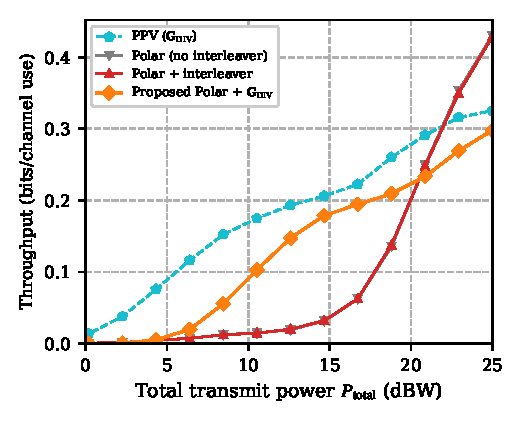
\includegraphics[width=0.7\columnwidth]{throughput_reliability.eps}\\
{\small \textbf{Fig.~\ref{fig:throughput}:} {\color{blue}Effective throughput versus total transmit power at $\epsilon = 40^{\circ}$ with $n_{\mathrm{s}} = 6$ subchannels. The diversity transform operates at effective rate $R_c \cdot \varrho/n_{\mathrm{out}} \approx 0.33$; per-subchannel baselines at $R_c = 0.5$. MRC and SC are rate-optimised at each power level.}}
\end{center}

The latency comparison in Section~V now reads:

\begin{quote}
``Fig.~\ref{fig:latency_comparison} demonstrates the latency advantage
of the diversity transform over {\color{blue}MRC, SC, and} the HARQ-CC baseline
in~\eqref{eq:harq_bler}--\eqref{eq:harq_latency}{\color{blue},
configured with $K_{\max} = 4$,
$T_{\mathrm{RTT}} = 20$~ms~\cite{3GPP38821}, and persistent
blockage across retransmission attempts.
Latency values are geometric means over channel realisations.
MRC combines LLRs from all non-blocked subchannels (effective SNR $= \sum_j \bar{\gamma}_j$), and SC selects the subchannel with the highest instantaneous SNR; both repeat the same codeword on every subchannel and therefore require $k_c$ times more channel uses to deliver the same message size.}
Despite
the chase combining advantage, the diversity transform consistently achieves
lower transmission latency than {\color{blue}all three baselines} across all operating points.
{\color{blue}For example, at $P_{\mathrm{total}} = 10$~dBW and $\epsilon_{\mathrm{sys}}^{\mathrm{target}} = 10^{-3}$, the diversity transform achieves approximately three times lower latency than HARQ-CC.}
As the target system BLER $\epsilon_{\mathrm{sys}}^{\mathrm{target}}$
becomes stricter, HARQ-CC latency grows faster because each
additional retransmission round adds a full round-trip time{\color{blue}, while MRC and SC latency grows because their per-subchannel codeword must be $k_c$ times longer to deliver the same message}.''
\end{quote}

\begin{center}
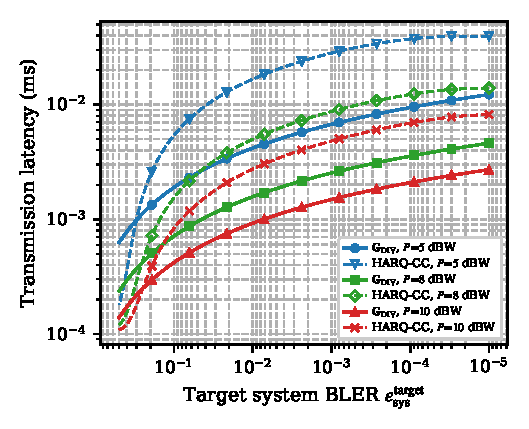
\includegraphics[width=0.7\columnwidth]{latency_comparison.eps}\\
{\small \textbf{Fig.~\ref{fig:latency_comparison}:} {\color{blue}Transmission latency versus target system BLER $\epsilon_{\mathrm{sys}}^{\mathrm{target}}$ for the diversity transform, MRC, SC, and HARQ-CC ($K_{\max} = 4$, $T_{\mathrm{RTT}} = 20$~ms) at $P_{\mathrm{total}} = 5$ and $10$~dBW. MRC and SC require $k_c = 4$ times more channel uses to deliver the same message size.}}
\end{center}

In addition to the MRC/SC/HARQ-CC comparisons above, the revised manuscript also demonstrates that the benchmarking results are not specific to a single FEC scheme. Fig.~\ref{fig:fec_comparison} evaluates the proposed architecture with both polar codes and LDPC codes at three code rates, confirming that the system-level performance is governed by the MDS erasure recovery rather than the choice of FEC decoder (see Comment~4 for detailed discussion). This addresses the reviewer's concern that the original manuscript compared only against isolated polar-coded baselines.

\begin{center}
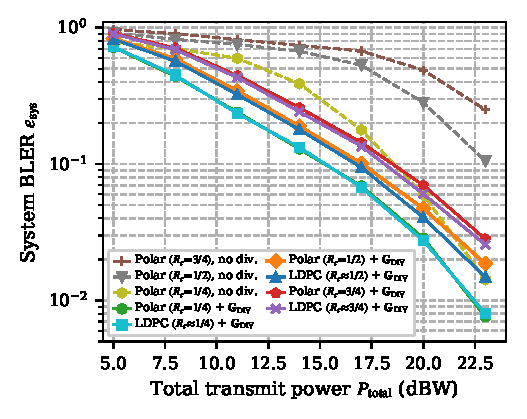
\includegraphics[width=0.7\columnwidth]{fec_comparison.eps}\\
{\small \textbf{Fig.~\ref{fig:fec_comparison}:} {\color{blue}System BLER versus total transmit power for polar and LDPC codes with the proposed diversity transform. No-diversity baselines shown for reference.}}
\end{center}

The summary paragraph in Section~V has been updated to reflect the expanded baseline set:

\begin{quote}
``$\ldots$ Finally, single-shot decoding eliminates the round‑trip latency associated with HARQ retransmissions {\color{blue}and achieves lower latency than MRC and SC baselines when normalised for equal message size} (Fig.~\ref{fig:latency_comparison}), consistent with the latency reduction established in Corollary~\ref{cor:latency_reduction}. This indicates that spatial diversity across co‑visible LEO satellites can replace temporal diversity via retransmissions.''
\end{quote}

The conclusion (Section~VI) now explicitly summarises the performance against all integrated baselines:

\begin{quote}
``{\color{blue}The diversity transform also outperforms MRC, SC, and HARQ-CC across latency and throughput metrics, overcoming the fundamental spectral efficiency ceiling of repetition-based combining.}''
\end{quote}

We note that a direct BLER comparison between MRC/SC and the diversity transform at equal message size and equal channel uses is mathematically impossible: MRC would require a code rate of $k_c \times R_c = 2.0 > 1$, which is unrealisable. This fundamental gap arises because MRC repeats the same codeword on all subchannels, while the diversity transform transmits different coded content. The throughput and latency comparisons are therefore the appropriate metrics for evaluating these integrated schemes.

We trust that the expanded benchmarking against MRC, SC, and HARQ-CC provides the system-level comparison requested.


\subsection{Reviewer Comment-6}



\begin{mdframed}
\begin{quote}
In Section III-A, the OTFS frame blocklength is defined as $n_c = N_D M_D$. Later, in Section IV-B, the Polar code blocklength is introduced as $N$ (i.e., an $(N, K)$ polar code), and $N$ is also used in Figure 7. It is not explicitly stated whether the Polar codeword length strictly matches the OTFS frame length (i.e., $n_c = N$), or if multiple Polar codewords are mapped onto a single OTFS frame. The authors should explicitly clarify this mapping relationship to prevent reader confusion regarding the system's frame structure
\end{quote}

\end{mdframed}


\subsection{Response}

We thank the reviewer for identifying this ambiguity. The relationship between the OTFS frame blocklength and the polar code blocklength is now explicitly clarified in Section~IV-B:

\begin{quote}
``{\color{blue} Each information subword is independently encoded into a polar codeword of length $N$. Accordingly, the channel-coding blocklength used in the finite-blocklength analysis of Section~\ref{sec:finite blocklength} is $n_c = N$, with each codeword occupying $N$ binary-modulated channel uses. For each subchannel, the OTFS frame contains $N_{\mathrm{D}} \times M_{\mathrm{D}}$ resource elements and carries $(n_{\mathrm{out}}/n_{\mathrm{s}})$ independently encoded transform outputs. This establishes the
interface between the diversity transform layer and the OTFS physical layer.}''
\end{quote}

To summarise: a single polar codeword of length $N$ constitutes one subword in the diversity transform, so $n_c = N$. The OTFS frame carries $(n_{\mathrm{out}}/n_{\mathrm{s}}) = 3$ such transform outputs per subchannel, each of length $N = 256$. A compact notation table (Table~\ref{tab:notation}) has also been added at the end of Section~I to allow readers to cross-reference all key symbols, including $n_c$, $(N,K)$, and $N_{\mathrm{D}}, M_{\mathrm{D}}$.

We hope that this clarification resolves the ambiguity between the frame and coding blocklengths.

\vskip 0.2in
We sincerely thank you for the thorough and constructive review. Your comments have been instrumental in strengthening the manuscript, and we believe the revisions comprehensively address all the concerns raised.
%%%%%%%%%%%%%%%%%%%%%%%%%%%%%%%%%%%%%%%%%%%%%%%%%%%%%%%%%%%%%%%%%%%%%%